\FloatBarrier
\let\supplementsubsection\subsection
\renewcommand{\subsection}{\FloatBarrier\supplementsubsection}

\section{Supplementary Methods and Results}

\subsection{Reading guide and result status}

This supplement distinguishes four statuses:
\begin{itemize}[leftmargin=*]
    \item \textbf{Primary/confirmatory}: interpreted under its recorded pre-specification.
    \item \textbf{Supporting}: informative but not licensed as a headline claim.
    \item \textbf{Undecidable or underpowered}: no directional conclusion is drawn.
    \item \textbf{Incomplete}: excluded rather than imputed.
\end{itemize}
The project contains several sequentially designed controls.
A later control answers its own specification and does not retroactively change a failed earlier test.

\subsection{Full behavioral rosters}

% Generated by scripts/build_assets.py. Do not edit by hand.
\begin{longtable}{@{}llrrrrl@{}}
\caption{Open-weight behavioral results. Human reference shapes are reported separately in \cref{tab:human-reference}.}\label{tab:open-full}\\
\toprule
Model & Type & Contrast & 95\% low & 95\% high & Degenerate & Cell order \\
\midrule
\endfirsthead
\toprule
Model & Type & Contrast & 95\% low & 95\% high & Degenerate & Cell order \\
\midrule
\endhead
OLMo-2-7B-I & instruct & -0.646 & -0.703 & -0.587 & no & inverted \\
Zephyr-7B & instruct & -0.551 & -0.603 & -0.502 & no & inverted \\
Mistral-7B-I & instruct & -0.473 & -0.510 & -0.438 & no & inverted \\
Gemma-2-9B-I & instruct & -0.408 & -0.464 & -0.353 & no & inverted \\
Tulu-3-8B & instruct & -0.401 & -0.442 & -0.361 & no & inverted \\
Qwen2.5-14B-I & instruct & -0.370 & -0.409 & -0.330 & no & inverted \\
Qwen2.5-3B-I & instruct & -0.247 & -0.275 & -0.220 & no & inverted \\
Qwen2.5-7B-I & instruct & -0.238 & -0.266 & -0.210 & no & inverted \\
Llama-3.1-8B-I & instruct & -0.202 & -0.232 & -0.173 & no & inverted \\
Qwen2.5-1.5B-I & instruct & -0.167 & -0.183 & -0.150 & no & inverted \\
Qwen2.5-14B & base & -0.126 & -0.139 & -0.112 & no & inverted \\
Qwen2.5-7B & base & -0.051 & -0.058 & -0.044 & no & inverted \\
Qwen2.5-0.5B-I & instruct & -0.050 & -0.061 & -0.040 & no & inverted \\
Qwen2.5-3B & base & -0.048 & -0.054 & -0.042 & no & inverted \\
Qwen2.5-1.5B & base & -0.013 & -0.018 & -0.007 & no & tied \\
OLMo-2-7B & base & -0.004 & -0.010 & +0.002 & no & tied \\
Mistral-7B & base & -0.003 & -0.005 & -0.000 & yes & tied \\
Gemma-2-9B & base & -0.000 & -0.002 & +0.001 & yes & tied \\
Qwen2.5-0.5B & base & +0.000 & -0.003 & +0.004 & no & tied \\
Llama-3.1-8B & base & +0.003 & -0.002 & +0.007 & no & tied \\
\bottomrule
\end{longtable}

\begin{table}[t]
\centering
\small
\caption{Complete clean closed-API behavioral reruns (v3; provisional pending archival provenance). Gemini-2.5-Pro was partial and excluded.}
\label{tab:closed-full}
\begin{tabular}{@{}lrrrl@{}}
\toprule
Model & Contrast & 95\% low & 95\% high & CI excludes 0 \\
\midrule
GPT-5.5 & +0.528 & +0.444 & +0.610 & yes \\
Claude Opus 4.6 & +0.336 & +0.236 & +0.432 & yes \\
Claude Sonnet 4.6 & +0.211 & +0.104 & +0.324 & yes \\
Gemini 3.5 Flash & +0.168 & +0.081 & +0.258 & yes \\
Gemini 2.5 Flash & -0.029 & -0.118 & +0.065 & no \\
Claude Haiku 4.5 & -0.163 & -0.215 & -0.106 & yes \\
GPT-4o-mini & -0.237 & -0.279 & -0.197 & yes \\
GPT-4o & -0.269 & -0.354 & -0.181 & yes \\
GPT-5.4-mini & -0.694 & -0.759 & -0.624 & yes \\
\bottomrule
\end{tabular}
\end{table}

\begin{table}[t]
\centering
\small
\caption{Joint BigToM and moral-judgment results for engaged open instruct models.}
\label{tab:bigtom-engaged}
\begin{tabular}{@{}lrr@{}}
\toprule
Model & BigToM false belief & Moral contrast \\
\midrule
OLMo-2-7B-I & 0.890 & -0.646 \\
Zephyr-7B & 0.835 & -0.551 \\
Mistral-7B-I & 0.815 & -0.473 \\
Gemma-2-9B-I & 0.935 & -0.408 \\
Tulu-3-8B & 0.855 & -0.401 \\
Qwen2.5-14B-I & 0.985 & -0.370 \\
\bottomrule
\end{tabular}
\end{table}

\begin{table*}[t]
\centering
\small
\caption{Post-training checkpoint dissection.}
\label{tab:stages}
\begin{tabular}{@{}llrrrr@{}}
\toprule
Family & Stage & Contrast & $\beta_{\mathrm{intent}}$ & $\beta_{\mathrm{outcome}}$ & Rating SD \\
\midrule
OLMo-2-7B & base & +0.002 & +0.005 & +0.003 & 0.058 \\
OLMo-2-7B & SFT & -0.586 & +0.096 & +0.682 & 0.351 \\
OLMo-2-7B & DPO & -0.652 & +0.102 & +0.754 & 0.396 \\
OLMo-2-7B & Instruct & -0.687 & +0.123 & +0.809 & 0.412 \\
Tulu-3-8B & base & +0.007 & +0.006 & -0.002 & 0.097 \\
Tulu-3-8B & SFT & -0.258 & +0.130 & +0.388 & 0.206 \\
Tulu-3-8B & DPO & -0.395 & +0.169 & +0.564 & 0.289 \\
Tulu-3-8B & RLVR & -0.398 & +0.167 & +0.564 & 0.289 \\
Zephyr-7B & base & -0.001 & +0.002 & +0.003 & 0.029 \\
Zephyr-7B & SFT & -0.150 & +0.022 & +0.172 & 0.168 \\
Zephyr-7B & DPO & -0.552 & +0.083 & +0.634 & 0.388 \\
\bottomrule
\end{tabular}
\end{table*}


\paragraph{Open table interpretation.}
The two open base models marked degenerate in the developmental-ladder source are near-constant raters for that comparison.
The mixed-effects analysis nevertheless reports an estimable four-cell ordering for all 20 stored model runs, yielding 14 inverted and six tied.
The table's contrast intervals are scenario-group bootstrap intervals.

\paragraph{Closed table interpretation.}
Every closed estimate is based on 298 stories, three templates, and five sampled ratings per story--template pair.
Gemini-2.5-Pro is partial and excluded.
The complete clean v3 estimates are provisional until their local source files receive archival provenance.
No closed model enters a hidden-state, probe, RSA, steering, or erasure claim.

\subsection{Human reference values}

\begin{table}[h]
\centering
\small
\caption{Human reference shapes used in the project. These are not item-matched ground truth for the 298-row corpus.}
\label{tab:human-reference}
\begin{tabular}{@{}llrrrrr@{}}
\toprule
Reference & Measure & Neutral & Accidental & Attempted & Intentional & Contrast \\
\midrule
Adult & normalized permissibility & 0.033 & 0.267 & 0.933 & 0.967 & $+0.666$ \\
Child 4--5 & digitized two-cell & -- & -- & -- & -- & $+0.240$ \\
Child 6--7 & digitized two-cell & -- & -- & -- & -- & $+0.500$ \\
Child 8+ & digitized two-cell & -- & -- & -- & -- & $+0.630$ \\
\bottomrule
\end{tabular}
\end{table}

The adult row is from Young et al.\ 2007 Experiment 1 ($n=10$) and uses a different 12-scenario set.
The child rows constrain only the attempted/accidental contrast and inherit digitization error.
Under the open deterministic protocol, all 18 non-degenerate profiles were at or below the youngest wrongness-reference contrast ($+0.240$).
The secondary punishment ladder yielded the same 18/18 count against its younger-child contrast ($+0.090$).
GPT-5.5's clean closed-model contrast of $+0.5278$ was above the digitized ages 4--5 and 6--7 wrongness contrasts but below the 8+ contrast of $+0.630$.
Because protocols, items, response measures, and scale types differ, these are descriptive placements rather than developmental-age assignments.

\paragraph{Independent booklet anchor.}
As a robustness check, the project parsed the open Theory of Mind Booklet dataset of 321 children ages 3--12 \citep{sotomayor2024dataset}.
The anchor uses neurotypical sessions and the source's exclusion flags; a first-session-only sensitivity analysis changes any age-band contrast by at most 0.047.
On wrongness items, booklet accidental-blame proportions decline from 0.398 to 0.142 to 0.010 across ages 4--5, 6--7, and 8+, close to the independently digitized Cushman values of 0.455, 0.200, and 0.060.
The booklet's intent limb is intentional harm, not attempted harm, so this agreement supports the developmental shape of accidental exculpation but is not substituted into the model ladder.

\begin{figure}[h]
    \centering
    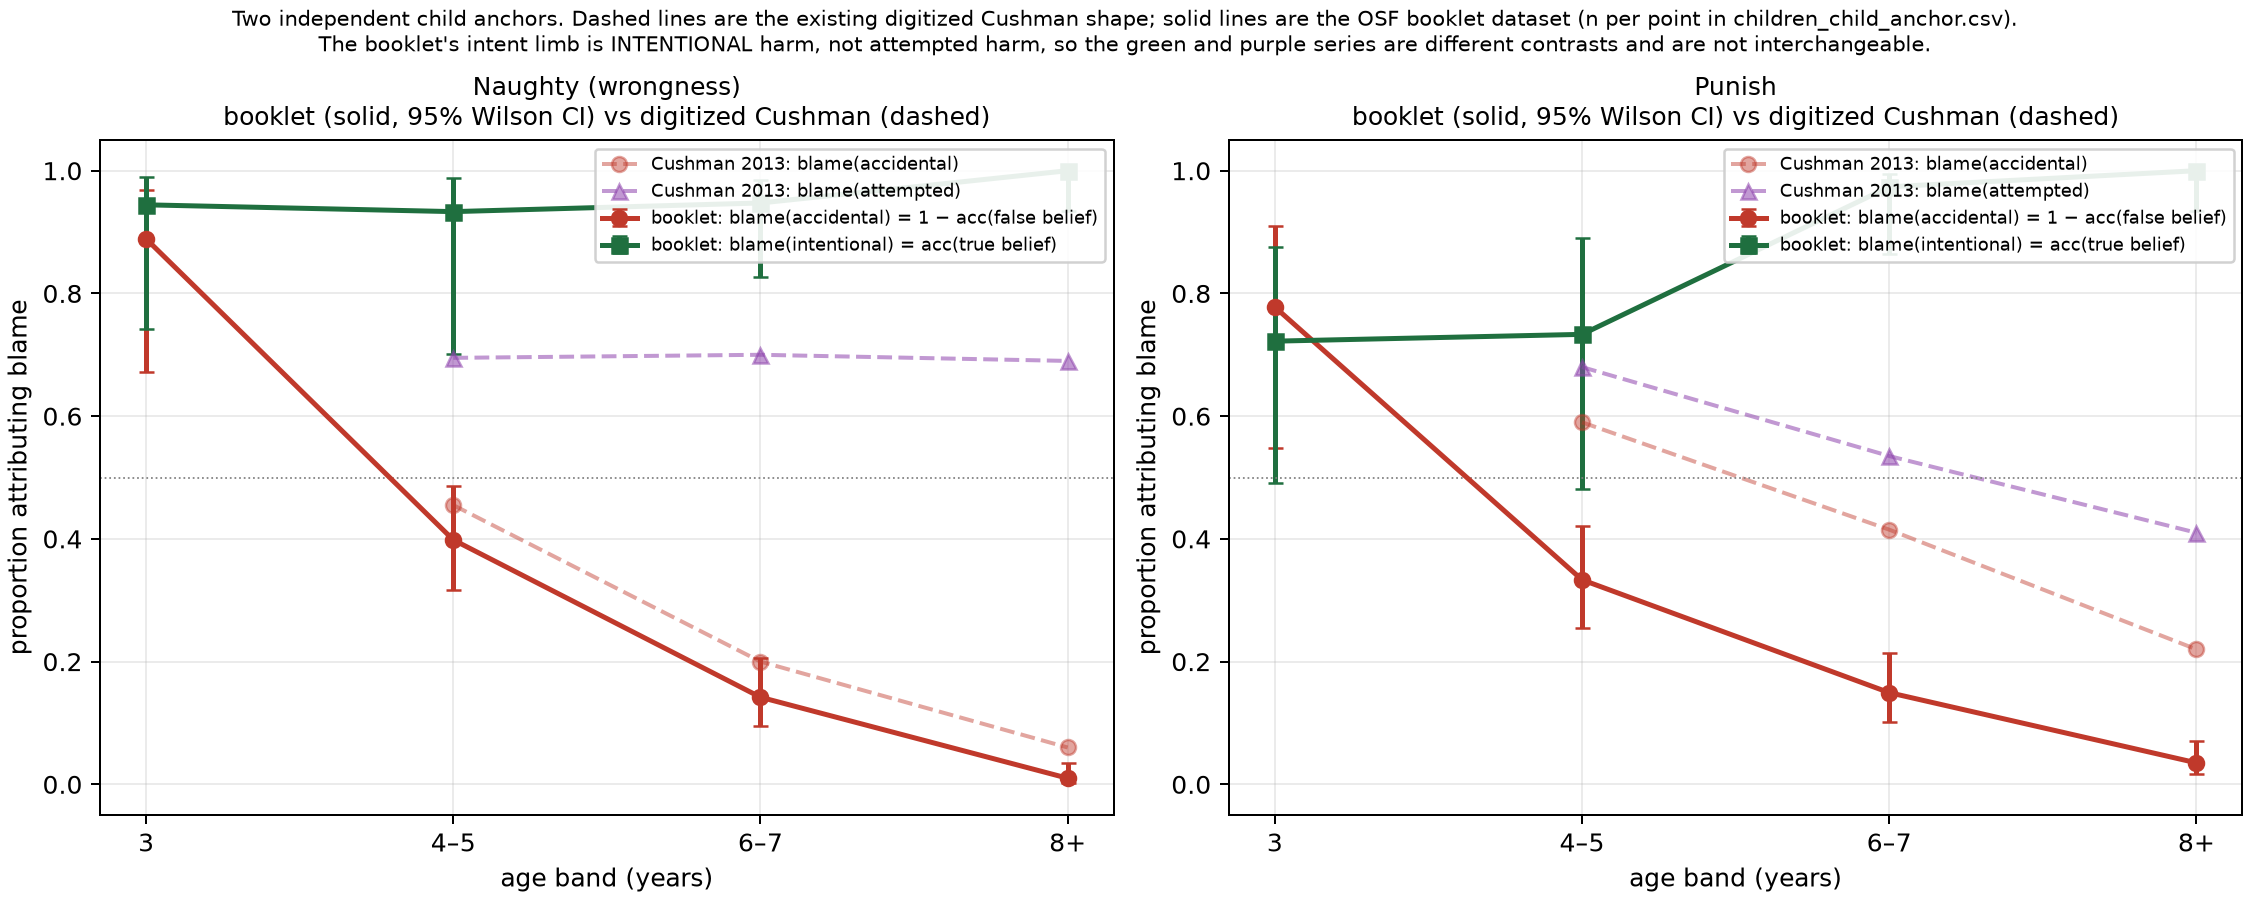
\includegraphics[width=\linewidth]{figures/child_anchor_booklet_vs_cushman.png}
    \caption{\textbf{Two independent child-reference shapes.}
    Solid lines are item-level booklet estimates with 95\% Wilson intervals; dashed lines are digitized Cushman series.
    The booklet contrast is intentional-minus-accidental and is not numerically interchangeable with the attempted-minus-accidental model contrast.}
    \label{fig:child-booklet}
\end{figure}

\subsection{Behavioral robustness and ancillary analyses}

\begin{table}[h]
\centering
\small
\caption{Supporting behavioral robustness results.}
\label{tab:behavior-robustness}
\begin{tabularx}{\textwidth}{@{}lXl@{}}
\toprule
Analysis & Result & Interpretation \\
\midrule
Common 1--7 prompts & 5/20 open models flip contrast sign & prompt sensitivity exists \\
Prompt construct variance & approximately 0\% in the project decomposition & wording/scale effects dominate construct label \\
EV versus sampling & correlation $>0.95$ for tested 7B instruct models & scoring parity supported in that slice \\
Qwen base$\rightarrow$instruct & mean paired shift approximately $-0.216$, paired $p\approx0.020$; Wilcoxon $p\approx0.063$ & family-specific evidence \\
Open scale versus contrast & Spearman $\rho\approx-0.23$, not significant & no scale claim \\
Source-scale agreement & pooled normalized correlation 0.71; bias $-0.06$; limits of agreement $[-0.44,+0.33]$ & cross-source averaging is imperfect \\
\bottomrule
\end{tabularx}
\end{table}

The two source instruments differ: the 2008 items use permissibility on a 1--3 scale and the 2009 items use blame on a 1--4 scale.
Normalization places both on a common condemnation direction but does not make the constructs identical.

\subsection{Measurement audits: normalization, clustering, story variance, and reliability}
\label{sec:supp-normalization}

The 2008 human scale (1 = forbidden, 3 = permissible) and the 2007 adult anchor run opposite to the model source-verbatim prompt; the 2009 (1--4 blame) and 2011 (1--7 wrongness) scales and all six factorial templates (1--7) share the model direction.
The mean of 11 open instruct models minus nine base models (2{,}000-resample scenario bootstraps) was $-0.319$ $[-0.345,-0.291]$ under endpoint scaling, $-0.309$ $[-0.334,-0.281]$ under per-model min--max, $-0.898$ SD $[-1.007,-0.786]$ under z-scores within model $\times$ template $\times$ source, and $-0.259$ $[-0.293,-0.225]$ under ranks; 9/9, 9/9, 7/9, and 8/9 pairs, respectively, were negative with intervals excluding zero.
Against endpoint scaling, the 34-entry model ordering had Spearman $\rho=0.996$, 0.945, and 0.946 with 0, 1, and 2 sign flips.
Under z-scores, the Qwen2.5-7B pair interval includes zero and Qwen2.5-14B reverses ($+0.19$ $[+0.03,+0.37]$), as it also does under ranks ($+0.05$ $[+0.005,+0.10]$); the ordering flips are OLMo-2-7B base and Gemini 2.5 Flash, both near zero under endpoint scaling.
Closed models enter the ordering without base partners, and Qwen chat-template-off reruns are separate entries excluded from class means.


\paragraph{Clustering and story variance.}
With Ward linkage and MDS on correlation distance between item rating profiles (20 models $\times$ 7 templates), outcome organized the item space (silhouette 0.30, adjusted Rand index 0.88), condition partly did (ARI 0.39), and intent (0.01, $\approx0$) and source (0.01, 0.07) did not; source clustering appeared only with the source-verbatim prompt (0.21, 0.22), where source and scale are confounded.
UMAP was not run.
Across the 20 open models, per-story variance in harm-outcome cells was about twice that of no-harm cells (accidental and intentional 0.081--0.087; attempted and neutral 0.036--0.043), and across-template variance was two to five times smaller (0.008--0.019).
In scenario-clustered regressions, accidental and intentional exceeded neutral by $+0.048$ ($p<10^{-4}$; $R^2=0.73$) and no clause-length term was significant (all $p>0.2$; across templates all $p>0.1$); the planned human-versus-model comparison was not run because the scanner data lack a story mapping.

\begin{table}[h]
\centering
\footnotesize
\caption{Spearman--Brown split-half reliability (median over 1{,}000 random splits; brackets are the 2.5--97.5\% split range). ``Within'' removes condition means first; model raters were z-scored within model $\times$ template $\times$ source.}
\label{tab:reliability}
\resizebox{\linewidth}{!}{%
\begin{tabular}{@{}lrrrr@{}}
\toprule
Raters & 2008 raw & 2008 within & 2009 within & 2011 within \\
\midrule
Templates (median of 20 models) & 0.94 & 0.89 & 0.92 & 0.93 \\
Instruct models (11) & 0.97 [0.95, 0.98] & 0.83 [0.76, 0.88] & 0.84 [0.77, 0.90] & 0.93 [0.83, 0.99] \\
Base models (9) & 0.59 [0.29, 0.68] & 0.36 [0.14, 0.52] & 0.59 [0.41, 0.72] & 0.64 [$-0.23$, 0.94] \\
MOR4 humans (13; story numbers) & 0.22 [$-0.31$, 0.56] & 0.39 [0.10, 0.61] & -- & -- \\
\bottomrule
\end{tabular}}
\end{table}

The 2011 rows contain only ten items, and no per-item human data exist for 2009 or 2011.
The human row uses unmapped story numbers with roughly six raters per half (story $\times$ condition cells: 0.69 [0.59, 0.80]).
Closed-model sampled ratings were identical across the five samples for nearly all items, so sample-level split-half values are uninformative and are not interpreted.

\paragraph{MOR4 scanner behavior.}
The MOR4 files are a scanner replication of the 2008 design (18 subjects, up to six runs of eight trials); conditions recovered from SPM onsets matched the stored trial order in every session checked.
Five subjects recorded no responses and 314 of 792 trials (39.6\%) lack a response; only three response keys were used, matching the 1--3 scale of the 2008 appendix rather than the 1--4 mapping applied.
No story-to-scenario mapping was found, and the belief/outcome codes (T, G) and button direction were inferred from the data (the all-neutral cell had the lowest mean, SD 0.26).
Under that coding, means on the key-minus-48 scale for the two presentation levels coded BF and OF were 3.35/3.55 (intentional), 3.04/3.15 (attempted), 2.44/2.45 (accidental), and 2.03/2.11 (neutral); attempted minus accidental is $+0.60$ and $+0.70$, or about $+0.30$ and $+0.35$ if the keys are a 3-point scale.
These values are descriptive only and are not compared with model items.

\subsection{Story ablations and variance decomposition}
\label{sec:supp-ablation}

Ablated stories were scored with the seven factorial templates in Qwen2.5-7B and Llama-3.1-8B base and instruct models: agent's name only (298 stories), text before the foreshadowing sentence (298), belief sentences deleted (298), and text up to the outcome sentence (288).
Prior strength is $|$rating $-0.5|$ and context sensitivity is the full-story minus ablated rating (four models, 53 scenarios, scenario-bootstrap intervals).
Base/instruct mean prior strength was 0.17/0.23 (name only), 0.17/0.24 (before foreshadow), 0.17/0.26 (belief removed), and 0.15/0.16 (outcome removed); instruct minus base was $+0.056$ [0.050, 0.061], $+0.059$ [0.037, 0.082], $+0.083$ [0.065, 0.101], and $+0.007$ [$-0.003$, 0.018].
Mean absolute context sensitivity was 0.06/0.29, 0.05/0.28, 0.02/0.13, and 0.02/0.07, with instruct-minus-base differences of $+0.238$ [0.219, 0.255], $+0.228$ [0.201, 0.257], $+0.112$ [0.093, 0.134], and $+0.050$ [0.043, 0.057].


The first two ablations are identical across conditions, so their contrasts are zero by construction.
Removing the belief roughly doubled the instruct contrasts (Qwen $-0.24\rightarrow-0.45$; Llama $-0.20\rightarrow-0.47$); removing the outcome sentence while keeping the foreshadow halved them ($-0.10$, $-0.11$), leaving a harm effect of 0.15; base contrasts stayed within $\pm0.08$.
In a full-story decomposition over 20 open models, seven templates, and 298 stories ($R^2=0.49$), Type I shares in entry order were condition 17.3\%, condition $\times$ base/instruct 11.0\%, base/instruct 10.1\%, and at most 2.4\% for any other term; the largest unique $R^2$ drop was condition $\times$ base/instruct (8.6\%).
Main effects nested in interactions have zero unique drop, so their shares depend on entry order.

\subsection{Explicit ToM comparison}

The joint BigToM table in \cref{tab:bigtom-engaged} is the primary RQ1 result.
The following analyses are retained to prevent a confounded correlation from being overinterpreted:
\begin{itemize}[leftmargin=*]
    \item The raw all-model false-belief/contrast correlation is a confound demonstration because both variables proxy base/instruct status and model size.
    \item Instruct-only partial correlation: $r=-0.473$, 95\% interval $[-0.776,+0.513]$, $n=11$; uninformative.
    \item Covariate-adjusted OLS: partial $r=-0.310$, interval $[-0.612,+0.158]$; ToM coefficient $-0.379$, $p=0.211$.
    \item Within-family deltas: $r=-0.160$, interval $[-0.824,+0.807]$, $n=9$; uninformative.
    \item ToMi is not a primary ToM measure because 82\% of the scored slice was audited as non-ToM.
\end{itemize}

\paragraph{Standalone closed-model BigToM.}
The project also contains generative BigToM runs for closed models.
They are reported descriptively and are not pooled with the open log-probability protocol or used for a post-hoc correlation with the clean v3 moral reruns.

\begin{longtable}{@{}lrrrrl@{}}
\caption{Closed-model generative BigToM inventory. Partial and failed runs are retained visibly rather than imputed.}\label{tab:closed-bigtom}\\
\toprule
Model & $n$ & All & False belief & True belief & Status \\
\midrule
\endfirsthead
\toprule
Model & $n$ & All & False belief & True belief & Status \\
\midrule
\endhead
Claude Haiku 4.5 & 400 & 0.953 & 0.975 & 0.930 & complete \\
Claude Opus 4.6 & 400 & 0.985 & 0.985 & 0.985 & complete \\
Claude Opus 5 & 127 & 0.992 & 0.986 & 1.000 & partial \\
Claude Sonnet 4.6 & 400 & 0.940 & 0.990 & 0.890 & complete \\
Claude Sonnet 5 & 397 & 0.972 & 0.985 & 0.960 & partial \\
Gemini 2.5 Flash & 400 & 0.970 & 0.980 & 0.960 & complete \\
Gemini 2.5 Pro & 234 & 0.974 & 0.992 & 0.957 & partial \\
Gemini 3.5 Flash & 400 & 0.965 & 0.980 & 0.950 & complete \\
GPT-4o-mini & 400 & 0.915 & 0.955 & 0.875 & complete \\
GPT-4o & 400 & 0.968 & 0.970 & 0.965 & complete \\
GPT-5.4-mini & 400 & 0.950 & 0.990 & 0.910 & complete \\
GPT-5.5 & 393 & 0.990 & 0.990 & 0.990 & partial \\
o3 & 329 & 0.991 & 0.994 & 0.987 & partial \\
o4-mini & 373 & 0.984 & 0.995 & 0.972 & partial \\
Gemini 3.1 Pro preview & 0 & -- & -- & -- & failed \\
\bottomrule
\end{longtable}

\subsection{Post-training stages}

The full 11-row stage table is \cref{tab:stages}.
Stage shares are:
\begin{table}[h]
\centering
\small
\caption{Share of each family's base-to-final contrast shift.}
\label{tab:stage-shares}
\begin{tabular}{@{}lrrl@{}}
\toprule
Family & SFT share & Later-stage share & Dominant measured stage \\
\midrule
OLMo-2-7B & 85.4\% & 14.6\% & SFT \\
Tulu-3-8B & 65.4\% & 34.5\% & SFT \\
Zephyr-7B & 27.0\% & 73.0\% & DPO \\
\bottomrule
\end{tabular}
\end{table}

The ratio $\outcomebeta/\intentbeta$ spans 3.0--7.7 across all non-base stages.
Final-stage ratios are 6.6 for OLMo, 3.4 for Tulu, and 7.7 for Zephyr.
The robust statement is that outcome grows several-fold more than intent at each non-base stage; the exact multiplier is recipe-dependent.

\subsection{Linear probes and surface baselines}

\begin{table}[h]
\centering
\small
\caption{Probe ranges and span-matched baselines across the eight core open checkpoints.}
\label{tab:probe-summary}
\begin{tabular}{@{}lrrr@{}}
\toprule
Read position & Intent probe & Outcome probe & Relevant TF--IDF baseline \\
\midrule
Belief-clause endpoint & 0.900--0.983 & 0.793--0.924 & 0.591 intent; 0.581 outcome \\
Final story token & 0.671--0.883 & 0.980--1.000 & 0.594 intent; 0.755 outcome \\
\bottomrule
\end{tabular}
\end{table}

At the belief endpoint, all eight models have a larger probe-minus-surface gap for intent than outcome; the mean difference is $+0.0871$ (sign-test $p=0.0078$).
This was downgraded from a temporal-process headline after manual inspection showed that setup sentences can state the scenario's ground-truth hazard before the annotated belief clause.
The foreshadow analysis below localizes that information to a single sentence.
The result supports semantic generalization beyond bag-of-words, not anticipation of unseen content.
The table's TF--IDF values use all 298 rows; on the 290-story clause-masked set of the foreshadow analysis, the belief-endpoint outcome baselines are 0.631 (word) and 0.572 (character).

\subsection{Follow-up decoding: foreshadow, held-out templates, and token-wise}
\label{sec:supp-foreshadow}

\paragraph{Outcome at the intention stage.}
Main-text values for the 14 checkpoints use 290 stories after the clause mask and 1{,}000 permutations; the character TF--IDF baseline was 0.572, peak-layer belief-endpoint accuracy reached 0.92, and fixed-depth accuracy at the action endpoint was 0.62--0.83.
In token trajectories at the last belief token (288 2008/2009 stories), peak outcome accuracy on the original text was 0.71/0.80 for Llama-3.1-8B base/instruct (layer 16), 0.77/0.81 for OLMo-2-7B (layer 16), and 0.73/0.73 for Qwen2.5-7B (layers 22/14), against same-text TF--IDF of 0.60 (word) and 0.59 (character), all $p=0.001$.
Without the foreshadowing sentence, the text through the belief was byte-identical between outcome partners in 100\% of items, so chance accuracy is structural and no permutation test was run; trajectories were extracted without chat formatting at a fixed subset of depths.

\paragraph{Held-out templates.}
\label{sec:supp-templates}
Activations were taken at the last prompt token of each template, with chat formatting for both Qwen models and Llama-Instruct (Llama base has no chat template); OLMo was not extracted.
In construct-held-out splits the source-verbatim template stayed in training; all splits were crossed with scenario-grouped folds, and TF--IDF used the full prompt with the same splits.
Within-minus-pair gaps (about 0.10--0.20 beyond relative depth 0.6) exceeded within-minus-construct gaps.

\begin{table}[h]
\centering
\footnotesize
\caption{Intent decoding at the last prompt token. Fixed layer is relative depth 0.65; all accuracies have permutation $p=0.001$ (null mean 0.50, null 95th percentile $\leq0.53$). Word TF--IDF: within 0.602, pair 0.596, construct 0.600; character TF--IDF: 0.555, 0.550, 0.543.}
\label{tab:templates}
\begin{tabular}{@{}lrrrrrr@{}}
\toprule
Model & Layer & Within & Pair & Construct & Within $-$ constr.\ ($p$) & Peak constr.\ (layer) \\
\midrule
Qwen2.5-7B & 18 & 0.647 & 0.568 & 0.635 & 0.012 (0.15) & 0.755 (22) \\
Qwen2.5-7B-Instruct & 18 & 0.750 & 0.580 & 0.680 & 0.070 (0.001) & 0.825 (21) \\
Llama-3.1-8B & 21 & 0.698 & 0.560 & 0.601 & 0.097 (0.001) & 0.639 (17) \\
Llama-3.1-8B-Instruct & 21 & 0.859 & 0.706 & 0.801 & 0.058 (0.001) & 0.814 (27) \\
\bottomrule
\end{tabular}
\end{table}

\paragraph{Token-wise decoding.}
Eight stories failed the clause mask and ten had non-monotone stage ends, leaving 280 per model.
At the layers of \cref{app-fig:time-decoding}, the pre-specified statistics (1{,}000-resample scenario bootstraps; all intervals exclude zero) were: intent rise across the belief clause 0.37--0.44 (TF--IDF 0.13); intent change from the belief end to late bins $-0.16$ to $-0.21$ (TF--IDF 0.00); late intent slope $-0.011$ to $-0.015$ per bin; pre-outcome outcome slope $-0.004$ to $-0.010$ per bin; and outcome jump at the outcome clause 0.14--0.31 (TF--IDF 0.04).
In temporal generalization, the intent code formed a block over the belief and early action bins, whereas background-trained outcome codes transferred only weakly to the outcome clause, which formed a separate late block.
The RDM intent coefficient fell from 1.54--1.95 in the action stage to 0.25--0.37 in the outcome stage, a steeper decline than decoding accuracy; the two measure mean-pattern distance and linear separability, respectively.
An initial run coded the interaction RDM so that it summed to a constant with the intent and outcome RDMs, making the coefficients unidentifiable; it was recoded as a 0/1 conjunction (rank 3), all six models were rerun, and only corrected values are reported.

\subsection{Representation--behavior links}

\begin{table}[h]
\centering
\footnotesize
\caption{Tests linking representation to behavior.}
\label{tab:representation-links}
\begin{tabularx}{\textwidth}{@{}XrrrrX@{}}
\toprule
Analysis & Estimate & 95\% low & 95\% high & $n$ & Status \\
\midrule
Item-level primary slope & $+0.0619$ & $-0.1463$ & $+0.2701$ & 384 & informative null vs $+0.30$ \\
Item-level matched slope & $+0.0291$ & $-0.1649$ & $+0.2231$ & 424 & informative null vs $+0.30$ \\
RSA pair link & $+0.0980$ & $-0.3102$ & $+0.4596$ & 28 pairs & null \\
Model-level probe link & $\approx-0.209$ & $\approx-0.80$ & $\approx+0.58$ & $\approx8$ & uninformative; footnote only \\
\bottomrule
\end{tabularx}
\end{table}

The RSA test asks whether models with more similar internal geometry have more similar moral contrasts.
Its interval admits moderate effects in either direction, so it is described as a null in the tested sample rather than proof of no relation.

\subsection{E1 variance partition: undecidable}

The pre-registered E1 gate required lexical unique variance to remain below the intent/outcome hypothesis RDMs before factor-specific unique variance could be interpreted.
All 36 designated model--layer cells were excluded under the full-document control, and all 36 were again excluded under a span-matched setup-only control.
The experimental factors are lexically realized and setup text nearly identifies scenario, so lexical distance is neither an independent nuisance nor removable without also removing design information.
E1's P1 and P2 therefore have no verdict.
The post-hoc 3--18$\times$ outcome/intent ordering is not promoted to confirmatory evidence.

\subsection{E2 checkpoint-stage RSA: withdrawn for power}

Across six OLMo/Tulu stage transitions, cross-stage RDM shift and absolute contrast shift correlated at $\rho=+0.870$, with a cluster-bootstrap 95\% interval $[+0.200,+1.000]$.
Despite the high point estimate, $n=6$ was pre-specified as underpowered; P1 was withdrawn.
Withdrawal is not evidence for the converse.
A Spearman--Brown correction was required before comparing observed RSA with the split-half ceiling.

\subsection{Additive steering details}

\begin{table}[h]
\centering
\footnotesize
\caption{Causal steering summary at coherent doses.}
\label{tab:steering-summary}
\begin{tabularx}{\textwidth}{@{}Xrrrr@{}}
\toprule
Model & Baseline $\contrast$ & Intent-probe max $|\Delta|$ & Outcome control max $|\Delta|$ & Resolution ratio \\
\midrule
OLMo-2-7B-Instruct & $-0.4452$ & 0.0128 & 0.2319 & 18$\times$ \\
Qwen2.5-7B-Instruct & $-0.2667$ & 0.0155 & 0.2592 & 17$\times$ \\
\bottomrule
\end{tabularx}
\end{table}

Manipulation checks:
\begin{itemize}[leftmargin=*]
    \item For OLMo, downstream intent-decoding accuracy changed from 0.893 to 0.500; the probe-margin displacement was $-3.18$ SD and $\Delta\contrast=-0.0128$.
    \item For Qwen, downstream intent-decoding accuracy changed from 0.899 to 0.500; the probe-margin displacement was $+7.21$ SD and $\Delta\contrast=+0.0056$.
    \item Both coefficient signs drive decoding toward chance, indicating off-manifold displacement rather than selective strengthening in one direction.
    \item At shallow layers the outcome control is at the random-direction floor; those cells are uninformative.
    \item At peak-intent and deeper resolvable layers, the probe-weight intent direction remains at or near the random floor while the outcome direction is effective.
\end{itemize}

Difference-of-means ``intent'' directions can raise all four cell means.
Because the accidental cell begins closest to the top of the scale, it has least headroom; the diagonal contrast then moves through ceiling compression.
Those movements are not treated as selective intent reweighting.

\subsection{Prose/rating dissociation}

Models were asked to explain a rating without being prompted to mention belief, intent, or accident; mention was coded by a primary coder and was not randomized.

\begin{table}[h]
\centering
\small
\caption{Ratings restricted to stories whose explanation names belief or intent, primary coder.}
\label{tab:prose}
\begin{tabular}{@{}lrrrrr@{}}
\toprule
Model & Mention rate & $n$ subset & $\intentbeta$ & $\outcomebeta$ & Ratio \\
\midrule
OLMo-2-7B-Instruct & 0.815 & 243 & $+0.078$ & $+0.444$ & 5.7$\times$ \\
Qwen2.5-7B-Instruct & 0.691 & 206 & $+0.026$ & $+0.310$ & 12.2$\times$ \\
\bottomrule
\end{tabular}
\end{table}

Lexicon-coded mention rates were 0.859 and 0.711.
Lexicon--hand-label Cohen's $\kappa$ was 0.725--0.756; lexicon--LLM-coder $\kappa$ was 0.423--0.488.
Surface mention is not evidence that the mentioned state is correct or causally used, and explanations are post-hoc to the rating.

\subsection{Prompt curriculum}

\begin{table}[h]
\centering
\small
\caption{Pre-registered L5 prompt-curriculum change from baseline.}
\label{tab:curriculum}
\begin{tabular}{@{}lrrl@{}}
\toprule
Model & Baseline & L5 & $\Delta$ and bar \\
\midrule
Zephyr-7B & $-0.552$ & $-0.337$ & $+0.215$, met \\
Qwen2.5-14B-Instruct & $-0.338$ & $+0.004$ & $+0.342$, met \\
Tulu-3-8B & $-0.398$ & $-0.325$ & $+0.073$, not met \\
OLMo-2-7B-Instruct & $-0.687$ & $-0.434$ & $+0.253$, met \\
Mistral-7B-Instruct & $-0.460$ & $-0.397$ & $+0.063$, not met \\
Gemma-2-9B-Instruct & $-0.375$ & $-0.265$ & $+0.110$, not met \\
\bottomrule
\end{tabular}
\end{table}

The pre-registered success rule required at least four of six models to clear $+0.15$; three did.
At L5, five of six improvements were attributable primarily to reduced accidental condemnation.
In the secondary ablation, principle-alone exceeded the full stack by more than 0.05 in three of six models, and all models were sub-additive across components.
Intent-led attempted-cell increases appeared clearly in two of six models under principle-alone.

\subsection{Outcome erasure and control sequence}

\begin{table}[h]
\centering
\small
\caption{Gate-passing outcome-erasure results.}
\label{tab:erasure-summary}
\begin{tabular}{@{}lrrrl@{}}
\toprule
Model & $\Delta\contrast$ & Cell-spread retention & Outcome removed & Label \\
\midrule
OLMo-2-7B-Instruct & $+0.3182$ & 0.5124 & yes & recovery \\
Qwen2.5-7B-Instruct & $+0.2312$ & 0.6697 & yes & recovery \\
Tulu-3-8B & $+0.3480$ & 0.3753 & yes & collapse \\
\bottomrule
\end{tabular}
\end{table}

\paragraph{Original specificity test (E5a).}
The matched-norm Qwen scenario perturbation moved $\contrast$ by $+0.1345$ at perplexity ratio 1.60, exceeding both the 0.0988 effect floor and the 1.5 coherence bound.
The pre-specification did not restrict P1 to coherent doses, so P1 remains failed.
Outcome/nuisance separation was 10.26$\times$ in OLMo, 1.72$\times$ in Qwen, and 4.31$\times$ in Tulu; the 2$\times$ bar failed in Qwen.
At coherent doses only, the largest Qwen nuisance movement was $+0.0929$ and separation was 2.49$\times$, but this is a secondary restatement.

\paragraph{Orthogonalized erasure (E6).}
With nuisance directions orthogonalized against outcome and intent and dose restricted to $s\leq1$, the largest coherent nuisance movement was 0.0160.
Minimum model-wise separation was 9.9$\times$, 22.3$\times$, and 24.6$\times$.
E6's absolute-floor conjunction held in only one of three models because the matched outcome arm was scaled to approximately one-third to one-half strength while tested against a full-strength floor.
The ratio-based P2 held in all three.
E6 is a new control, not a reversal of E5a.

\paragraph{Symmetric residual control (E7b).}
At matched displacement:
\begin{itemize}[leftmargin=*]
    \item OLMo's scenario-orthogonal outcome arm moved $\contrast$ by $+0.1549$ and its full outcome control by $+0.1880$: A-shaped.
    \item Qwen's test arm moved $+0.0322$ and its positive control $+0.0630$, both below the 0.0988 floor: void.
    \item Tulu's test arm moved $+0.0941$, 95\% of the floor, while its positive control moved $+0.1420$ and its complement $+0.1008$: assigned to the pre-registered falsifier branch, but near the threshold.
\end{itemize}
The split authorizes no pooled outcome-specific claim.

\subsection{Cross-domain harm-code support}

The project-local Bruneau stimulus set uses 144 items in 72 matched pairs across physical pain, emotional suffering, and false-belief harm \citep{bruneau2012shared}.
Its local filename uses 2011, consistent with the article's December 2011 online publication; the journal issue and bibliography year are 2012.
It does not contain attempted-harm conditions and therefore cannot test intent weighting.
Within-domain harm decoding was often 0.9--1.0.
At a single selected layer per model, mean within-domain versus cross-domain decoding was 0.951 versus 0.771 for Qwen and 0.979 versus 0.809 for OLMo.
Substantial cross-domain transfer supports a largely shared harm representation while leaving the intent-use question open.

\subsection{Checkpoint emergence}

\begin{table}[h]
\centering
\small
\caption{End-of-trajectory RDM coefficients and behavioral engagement.}
\label{tab:e8-summary}
\begin{tabular}{@{}llrrl@{}}
\toprule
Family & Read position & $\beta_{\mathrm{intent}}$ & $\beta_{\mathrm{outcome}}$ & Gradeable checkpoints \\
\midrule
Pythia-1.4B & belief endpoint & $+0.1042$ & $+0.0003$ & 0/26 overall \\
Pythia-1.4B & story end & $-0.0065$ & $+0.4899$ & 0/26 overall \\
OLMo-2-7B & belief endpoint, depth .8 & $+0.108$ & $+0.010$ & 0/20 stage-1 \\
OLMo-2-7B & story end, depth .8 & $+0.021$ & $+0.494$ & 0/20 stage-1 \\
\bottomrule
\end{tabular}
\end{table}

Pythia details:
\begin{itemize}[leftmargin=*]
    \item 26 checkpoints, step 0 through 143{,}000.
    \item Step-0 gate passed: 0/20 intent/outcome predictor cells outside even the uncorrected 95\% band.
    \item The registered prediction that outcome would emerge before intent at the primary belief-endpoint cell failed; the cell was structurally unsuitable for that ordering test.
    \item The registered non-decreasing outcome-share prediction failed at the primary cell ($\rho=-0.639$, interval $[-0.935,-0.113]$).
    \item Shape verdicts across the primary specification were 17 smooth, two indistinguishable, and one breakpoint.
    \item Peak rating SD was 0.0859 against the 0.2191 floor.
\end{itemize}

OLMo details:
\begin{itemize}[leftmargin=*]
    \item 20 stage-1 revisions, steps 150 through 928{,}646.
    \item At the final stage-1 revision, the target/off-target pattern held at 5/5 belief-endpoint depths and 4/5 story-end depths; the replication criterion was at least 3/5 at each position.
    \item At depth 0.8, onset is bracketed between step 1{,}000 (approximately 5B tokens, inside null) and step 2{,}000 (approximately 9B tokens, clear).
    \item Sigmoid fits were preferred for belief-endpoint intent ($\Delta\mathrm{AICc}=5.504$, $R^2=0.9077$) and story-end outcome ($\Delta\mathrm{AICc}=30.988$, $R^2=0.9839$).
    \item No random-initialization checkpoint is published for this family.
    \item The joined trajectory has two seams: stage-1 activations were extracted in float32 while stage activations used float16, and stage-2 annealing is unsampled.
\end{itemize}

The Pythia and OLMo step indices are not directly comparable.
Approximate token counts place Pythia story-end outcome at approximately 2.1B tokens and belief-endpoint intent at approximately 6.3B, while OLMo brackets both at 5--9B.
Only order-of-magnitude similarity is claimed.

\subsection{Cross-cultural placement}
\label{sec:supp-crosscultural}

The cross-cultural comparison uses a different axis---intentional minus accidental at constant harm---because the ten-society dataset has no failed-attempt cell \citep{barrett2016societies,curtin2020kinship}.
Nine of ten societies had positive badness effects with intervals excluding zero; Yasawa was $0.0000$ [${-0.0265},+0.0227$].


\begin{table}[h]
\centering
\small
\caption{Badness intent effects at constant harm in ten societies.}
\label{tab:societies}
\begin{tabular}{@{}lrrr@{}}
\toprule
Society & $n$ subjects & Scaled effect & 95\% CI \\
\midrule
Storozhnitsa & 28 & $+0.2411$ & $[+0.1786,+0.3036]$ \\
Los Angeles & 39 & $+0.2115$ & $[+0.1282,+0.2949]$ \\
Sursurunga & 20 & $+0.2000$ & $[+0.0500,+0.3375]$ \\
Martu & 18 & $+0.1944$ & $[+0.0556,+0.3194]$ \\
Karo Batak & 30 & $+0.1833$ & $[+0.0833,+0.2917]$ \\
Hadza & 29 & $+0.1379$ & $[+0.0690,+0.2155]$ \\
Shuar & 34 & $+0.1324$ & $[+0.0072,+0.2574]$ \\
Himba & 24 & $+0.1146$ & $[+0.0417,+0.1979]$ \\
Tsimane & 32 & $+0.1016$ & $[+0.0156,+0.1955]$ \\
Yasawa & 66 & $+0.0000$ & $[-0.0265,+0.0227]$ \\
\bottomrule
\end{tabular}
\end{table}

The engaged-model count is 4/6 below the literal lowest society and 6/6 below the lowest society with a detectable positive effect.
For all 18 non-degenerate open models, the corresponding counts are 12/18 and 18/18.
The society intervals are over subjects, whereas deterministic model points have no commensurate subject-level uncertainty.

\subsection{Stimulus and measurement provenance}

The pre-repair parser appended rating prompts and parts of subsequent scenarios to selected harm cells.
Three counters must not be conflated: 144 regex-detector hits, 96 of 154 harm cells in the per-condition table, and 99 visible trailing artifacts in the archived CSV.
Repair changed 260 of 298 rows and recovered names/backgrounds for all 48 2008 scenarios.
An independently discovered CPR polarity inversion was corrected by deriving action polarity from text and audited manually.

Every pre-repair result was regenerated.
The project preserves a checksum-addressed contaminated master and quarantined outputs rather than deleting them.
The current validation script has ten hard checks and exits non-zero on failure.

Three measurement failures motivated the no-imputation rule:
\begin{enumerate}[leftmargin=*]
    \item a digit-token mapping failure that returned the scale midpoint;
    \item a coherence detector that rejected valid single-digit outputs; and
    \item a closed-API parser that wrote midpoint ratings for failed calls.
\end{enumerate}
A failed measurement is now missing and must carry an answer/parse status.

\subsection{Reproducibility boundaries}

Scenario-group bootstraps use 2{,}000 replicates and seed 0 in the shared resampler.
The item-level slope uses 10{,}000 item resamples; the ToM comparison uses 10{,}000 model resamples; RSA convergence uses 1{,}000 pair resamples.
The E6 rebuild reproduces the committed L40S outputs bit-exactly on matched hardware.
On A100 hardware, perplexity ratios differed by up to 0.031, contrast by at most 0.002, and no gate decision changed.

Raw activations are gitignored and must be regenerated.
Package-lock or container metadata sufficient to recreate the complete software environment is \missinginfo.
The public archival identifier for the clean closed v3 data is also \missinginfo.

\subsection{Excluded and incomplete measurements}

\begin{itemize}[leftmargin=*]
    \item Gemini-2.5-Pro closed behavioral run: partial; excluded.
    \item Closed reasoning-dose study: incomplete; no clean figure; excluded.
    \item Contaminated-era closed moral contrasts: quarantined; excluded.
    \item Stale combined open/closed ladder figures: excluded.
    \item ToMi primary comparison: excluded after slice-content audit.
    \item Missing coefficients at unengaged pretraining checkpoints: retained as missing, never plotted at zero.
\end{itemize}

\section{Claim Boundary Checklist}

The following formulations are licensed by the available evidence:
\begin{itemize}[leftmargin=*]
    \item ``Explicit false-belief success is insufficient evidence of applied intent use in the tested open models.''
    \item ``Intent is linearly decodable in the tested open checkpoints, while the tested representation--behavior links are null or uninformative.''
    \item ``Probe-weight intent steering is small relative to an outcome-direction positive control at resolvable depths in two models.''
    \item ``Outcome erasure produces the pre-registered recovery signature in two of three models.''
    \item ``SFT is sufficient in three public pipelines, while stage share is recipe-dependent.''
    \item ``Representational structure develops smoothly in the measured Pythia and OLMo trajectories; pretraining checkpoints are not behaviorally gradeable under this rating assay.''
    \item ``Intent decoding transfers to held-out rating constructs in two base/instruct pairs.''
    \item ``Outcome decodability at the belief endpoint reflects the foreshadowing sentence.''
\end{itemize}

The following formulations are not licensed:
\begin{itemize}[leftmargin=*]
    \item ``All LLMs fail intent-sensitive moral judgment.''
    \item ``No model reaches an eight-year-old level.''
    \item ``Outcome weighting is outside the human range.''
    \item ``The intent representation is causally inert at every layer or in every form.''
    \item ``Only the outcome direction controls judgment.''
    \item ``SFT rather than preference optimization causes the bias in every recipe.''
    \item ``The belief endpoint is outcome-free'' or ``the model predicts an unseen outcome.''
    \item ``The MOR4 scanner data provide an item-matched human reliability or variance benchmark.''
    \item ``Instruction tuning lowers the contrast in every model family'' or ``base and instruct models differ in template generalization in general.''
    \item ``Passing or matching behavior establishes genuine, conscious, or human-like ToM.''
\end{itemize}
